\documentclass[12pt, conference, a4paper]{article}
\usepackage{a4wide}
\usepackage[centertags]{amsmath}
\usepackage{amsfonts,amssymb,amsthm}
\usepackage{graphicx}
\usepackage{wrapfig}
\usepackage{iitbcstitle}
% \usepackage{listings}
% \usepackage{xcolor}
% \usepackage{xparse}
\usepackage[cache=false]{minted}
\usepackage{biblatex} 
\usepackage{url}
\usepackage{hyperref}
\usepackage{todonotes}
\usepackage[none]{hyphenat}
\usepackage{enumitem}
\usepackage{booktabs}
\usepackage{float}
\linespread{1.15}
\usepackage[cm]{fullpage}
\usepackage{rotating}
\usepackage{times}
\usepackage{textcomp}
\setlength\parindent{0pt}
\addbibresource{references.bib}

\begin{document}

\title{APRICOT and SAFE\\
}
\author{
\begin{tabular}{c}  {Bhaveshkumar Yadav} \\ bhaveshy@iitb.ac.in \\Department of Computer Science \& Engineering \\ IIT Bombay \end{tabular} }

\maketitle
\pagenumbering{arabic}



\section{Introduction}
\label{SEC:introduction}
This report is the documentation of the work done on the SAFE and APRICOT app for iOS during the spring semester of 2019-20. SAFE (Smart, Authenticated, Fast Exams) is an application system used in IIT Bombay and 30+ other colleges for conducting exams, tracking attendance, online correction of regular exams, etc. 
APRICOT (A PRIvacy preserving COntact Tracing app) is a contact tracing app developed during the COVID-19 Pandemic to track the possible spread of infection. This documentation will help people pick up the project in the future. 
Section \ref{SEC: 1} describes the work done on Web Sockets for SAFE- iOS. Section \ref{SEC: 2} is about the periodic submission of a quiz in the background. Section \ref{SEC: 3} is the documentation of the iOS front-end APRICOT app, including details about Bluetooth scanning.

\section{SAFE - Websocket in iOS}
\label{SEC: 1}
In the Android version of the SAFE app, during an ongoing quiz, a WebSocket connection is established with the back-end. This connection is used to send real-time information to the server. For example, when a student puts the app in the background, the corresponding flags are immediately sent to the server.
Thus a teacher can view the real-time flags on the SAFE analytics dashboard. 
However, this feature is not implemented in the iOS app. The app logs information during the quiz locally. This information is only sent to the server when the quiz is submitted. Thus, while the quiz is going on, real-time data is not available from the iOS version of the app. 
My first task was to implement this feature in iOS. I started exploring various WebSocket libraries for iOS. 
\subsection{About WebSockets in iOS.}
WebSocket was not a first-class citizen in iOS before iOS 13. Hence to implement WebSockets reliably and conveniently, we needed to use third-party libraries. One of the most popular libraries is \textbf{Starscream}. It does all the heavy lifting behind the scenes and makes it easier to manage WebSockets. The library is open source and is available on \href{https://github.com/daltoniam/Starscream}{Github}\\
However, from iOS 13 onwards, WebSockets became a first-class citizen and can be easily implemented using URLSession. 
But to support older versions of iOS using Starscream was necessary.
\subsection{Starscream}
\subsubsection{Installation}
\begin{itemize}
  \item Add \textbf{pod 'Starscream', '\url{~>} 4.0.0'} at the end of the podfile
  \item Run \textbf{pod install} in the terminal
\end{itemize}
\subsubsection{Usage}
Import the library at the top of the swift file with \mintinline{swift}{import Starscream}\\
Once imported, we can open a connection to a WebSocket server as follows:
\begin{minted}{swift}
  var request = URLRequest(url: URL(string: "http://localhost:8080")!)
  request.timeoutInterval = 5
  socket = WebSocket(request: request)
  socket.delegate = self
  socket.connect()
\end{minted}
Note that socket should be a class property defined at the beginning of class as \mintinline{swift}{var socket:WebSocket!}\\

We are setting the current class as the delegate of the WebSocket class. Hence we must mention it in the class definition as follows:
\begin{minted}[]{swift}
  class  YourClass : WebSocketDelegate {
    ....
  }
\end{minted}

\begin{figure}[!htbp]
\begin{center}
  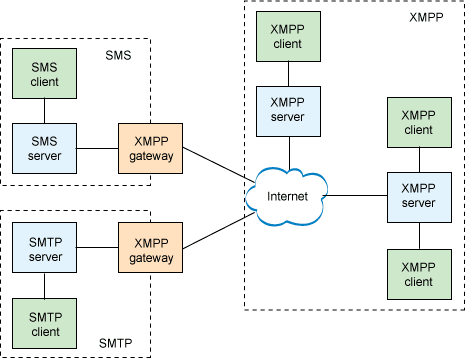
\includegraphics[width=3in]{xmpp_architecture.png}
\caption{XMPP architecture \cite{xmpp-arch}}
\label{fig: xmpp} 
\end{center}
\end{figure}
Figure \ref{fig: xmpp} illustrates the architecture.\\
XMPP server is responsible for connection management and message routing. The Gateway acts as a bridge between different networks. The underlying connection is TCP. The link is used for streaming XML data. A single TCP connection can carry multiple sessions. The Addressing scheme used is similar to that of e-mail. There is a unique address per device and not per user. The address is called Jabber Identity. It is of the form, \textit{user@domain/resource}. For example, \textit{lucifer@htl.hut.fi/phone}. Thus if a user has multiple devices, the message is routed to the specific equipment which he is using right now.
\par
The primary payload in XMPP is exchanged using XML. There are three primitives called XML stanzas defined in XMPP.
\begin{enumerate}
    \item \textbf{$<$message/$>$:} This stanza is used to carry message info and body
    \item \textbf{$<$presence/$>$:} This stanza is a broadcast that carries presence information about a user to his contacts who have subscribed to him. (Info like when the user is online )
    \item \textbf{$<$iq/$>$:} This stanza is used to carry requests and responses. For example, file transfer or contact list retrieve. 
\end{enumerate}
\par
Characteristics of XMPP:
\begin{itemize}
    \item Messages are stored before being forwarded. Thus XMPP implementations can keep messages for delivering later if the recipient is offline.
    \item The resource location is attached to the address itself. There is no need for an additional protocol to handle this.
    \item The underlying connection is TCP, which guarantees delivery.
    \item Presence information support is explicit in the standard with the presence stanza.
    \item Security has been taken into consideration too. Transport Layer Security (TLS) is used to achieve confidentiality and data integrity. Simple Authentication and Security Layer protocol (SASL) is used for authentication.
    \item The server-to-server federation is a feature that enables interoperability among different XMPP implementations. An essential feature for an open messaging standard.
\end{itemize}

\subsection{XMPP Extensions}
XMPP extensions are used to enhance the core functionalities of XMPP. These extensions are either produced and managed by Jabber Software Foundation(JSF) or by various research work and implementations. In the former case, they are called JEPs. The JSF follows a standard process while developing and approving these JEPs.
\par
Extensions make XMPP more attractive; it promises long life to the standard because new features can be added with time. Following is the list of popular extensions \cite{xmppEXT}.
\begin{itemize}
\item \textbf{Data Forms XEP} is used to specify data required to render forms on the client-side and the related semantics for forms processing( like request, response, submit and cancel )
\item \textbf{Multi-User Chat XEP} defines features required to support group chat and rooms. 
\item \textbf{Jingle XEP} extension is used to support media sessions like voice and video chat, file transfer, etc. This extension uses XMPP for the signaling required to set and manage these sessions. Google Talk used this extension. 
\item \textbf{Jabber-RPC XEP} defines how to transport RPC(Remote Procedure Calls) payload over XML. 
\end{itemize}
If a company doesn’t find an extension for its use case it can always define its own extension and add it to the standard as well. 

\subsection{XMPP implementations}
\begin{itemize}
\item The first IM service, which was based on XMPP, was Jabber.org, which started in 1999. In January 2010, the service migrated to a proprietary software called M-Link from Isode Ltd.
\item Google introduced Google Talk, which was a combination of VoIP and IM system that uses XMPP for instant messaging. It also used XMPP for signaling during file transfer and voice calls. In May 2013, Google dropped XMPP compatibility for server-to-server federation.
\item In February 2010, Facebook opened up its chat feature to third-party applications via XMPP. However, its support was dropped in April 2014.
\item In 2008, AOL introduced XMPP for the AOL Instant Messenger service, which was discontinued soon.
\item Whatsapp, the instant messaging giant, also initially began with XMPP but later switched to another proprietary protocol. \cite{xmpp-whatsapp}
\end{itemize}
Looking at the history of XMPP deployments, we can reasonably conclude that many companies have moved away from XMPP after using it for a while. Some applications still use XMPP for non-messaging purposes. But in the Instant Messaging sector, XMPP does not seem to be a widely accepted standard these days.

\subsection{Reasons for XMPP's downfall}
\begin{itemize}
\item When companies use XMPP as their architecture backbone, the user data is not directly present with the companies because it is a distributed system. A user might be using the service from some other client in which case the company doesn’t own the user’s data.
\item XMPP was designed to provide a way for chat networks to interoperate, known as federation. Google Talk was the only major app to support the federation, and even after a long time, the rest of the industry was not moving to embrace this open system. Open systems don't work if big companies don't support them.
\item The format used in XMPP message envelopes was strict, and it was too hard to break its role based on project requirements.
\item XMPP did not support end-to-end encryption. Efforts were made to add end-to-end encryption to the standard using extensions, but they were too late and did not gain popularity.
\end{itemize}
In the case of big corporations like Facebook and Google, the advantages of using XMPP are minimal; they won't have a problem building their own protocol.\\
Using XMPP will have the following disadvantages
\begin{itemize}
\item They won't be able to control user experience since there would be a large number of clients from different companies.
\item In the case of communication outside the network, they will have to deal with buggy servers and all kinds of configurations.
\item If they ever want to monetize by using ads, they will have a hard time since people can always switch to some other client.
\end{itemize}
Other reasons:
\begin{itemize}
\item With other apps, only the phone number is needed, while an XMPP user has a jabber ID, Which is associated with a device. A user may be using the service on the phone, computer, or some other device. A message sent to one device does not reach the other and leads to inconsistent chat history.
\item There is no QoS. Messages may not get delivered. They may get dropped, and the server might still show that they got delivered.
\item The group chat feature is not very efficient. They have defined a very complex implementation that is not used in modern apps. Even if apps don't use the feature, it still exists as a dead code.
\item The standard for file upload was way too late. It was first drafted in 2015.
\item XMPP uses XML which is too verbose for mobile environments that face problems like frequent disconnection and slower speeds. 
\end{itemize}
So we see that XMPP seemed promising as an open standard for instant messaging. Some big players supported it in the initial days, but now most of them use their own modified versions of the standard.

\section{Rich Communication Services (RCS)}
\label{SEC: rcs}
Rich Communication Services (RCS) is a communication protocol between mobile devices. It is the successor of SMS(Short Message Service) It primarily aims to bring Instant Messaging like features on traditional messaging infrastructure (SMS) of telecoms. Features like group chat, read and typing indicators, sending images, videos, and stickers.\\
\textit{How is it different from other messaging applications?}\\ In applications like Whatsapp and Facebook messenger, a single company manages and owns the user data. On the other hand, RCS (and SMS) is a federated system where multiple companies maintain servers and interoperate with each other. Once all manufacturers and service providers start supporting it, RCS features will be available through the SMS application, which comes pre-installed on all phones. The user does not need to download an additional app. Thus people won't need to ask their friends and family to join a new IM network. RCS standard was first introduced in the year 2007, but it has been adequately standardized only in the year 2016 by GSMA. \cite{rcs-wiki} \\
Carriers and device manufacturers have started supporting RCS. However, carriers have been very slow in doing so. Hence Google now provides RCS features through its servers instead of waiting for carriers to support it. The service can be used through Google's messages app, which comes pre-installed on a lot of Android phones. However, once telecom operators start supporting RCS fully, users can be shifted back to their servers. Samsung supports RCS through its messages app. However, it relies on telecom operators to support RCS too.\\
Apart from the peer to peer messaging feature, there is another feature in RCS, which is important. It's the Business to People messaging feature. Using RCS, businesses can directly reach their customers. And unlike SMS, RCS will allow them to embed dynamic content like interactive polls, forms, and direct payment flow. Thus businesses can benefit a lot from RCS. Company verified accounts could be used to provide customer support with automation.\\
RCS seems like an ideal candidate for an open messaging standard. It works out of the box, supports interoperability, has the promise of eventually getting everyone on board, supports rich content, and is backed up by big companies.\\
However, RCS may not gain popularity and user adoption because:
\begin{itemize}
\item RCS does not support end-to-end encryption (because telecom operators need to provide lawful interception to authorities when required) while most of the IM apps support it.
\item Proper interoperability among carriers is an issue.
\item Apple has not revealed any plans to support RCS. It already has iMessage, which has similar features but only for Apple devices. It may not support RCS in the future to avoid competition with iMessage. As long as Apple does not support RCS, it won't become universal.
\item RCS is a standard. It's not an application. User experience will depend on the client that the users will use.
\end{itemize}
Also, open messaging and interoperability may not be the motive behind companies supporting RCS. \cite{rcs-google} \\
Let's consider the architecture of Google's RCS platform.
Google's RCS Hub has three parts
\begin{enumerate}
\item The client App (Google messages)
\item Jibe RCS-cloud services platform: so that operators can do a simpler and cheaper setup of RCS on their network.
\item RCS Hub for interoperability among carriers.
\end{enumerate}
Through the RCS Hub, Google is providing a way for carriers to interoperate. Operators who aim to connect to other operators for interoperability need not connect to each operator separately. If they all connect to Google's RCS Hub, their efforts on interoperability will be reduced considerably.
For Google, the HUB will be an entry point for advertisements. Businesses who want to reach their customers through RCS can do so by connecting to the Google RCS HUB. \\
Hence Google's main aim with RCS may be to support its AD business. 
However, Google might not succeed with this plan as long as RCS does not become universal. If Apple doesn’t support RCS, businesses will not be able to reach the Apple customer base through RCS. Using other platforms like Whatsapp Business will be a better deal for them. 
\par
In conclusion, RCS looks very promising initially due it's interoperability, but the lack of crucial features (e2e encryption)and limited support (no support from Apple yet) make it less attractive.
\section{Other Efforts}
\label{SEC: other}
We have so far reviewed two significant standards. These were directly related to messaging and interoperability. Next, we will summarize a few efforts towards user privacy, countering fake news, network security, etc. which are closely related to the open messaging aim. \\
Current Social Networking Systems are centralized in terms of data ownership. All the data resides on the servers of the social media platform. These platforms capitalize on users' data. We discuss two proposed systems which aim to decentralize the data ownership.
\subsection{SOLID}
SOLID (derived from “social linked data”) is a new open-source project led by Prof. Tim Berners-Lee at MIT. \cite{SOLID} The project aims at providing true data ownership as well as improved privacy to the user. It promotes a modular design in which the data is decoupled from the applications. This will enable users to seamlessly switch from one app to another without losing any data and connections.  Within the SOLID ecosystem, the user decides where he stores his data. (Ex: Photos, comments, contacts) He can store it either on verified third party servers or on his own machine. To store the data on his machine he will need to install required softwares and follow the procedures listed on the website. This data is called the users' SOLID POD.  In order to write or read the data from the users POD, permission is required. The permission is managed using the web access control list specification. The POD should have a unique ID for which the WebID Identity spec is used. It allows a URI to denote a user. The user permits to read or write parts of his POD while signing up on an application. He then inputs the unique URI of his pod.   For security and authentication WebID-TLS and WebID-OIDC are used right now. Other strategies like two factor authentication could be added if needed.
\par
The data of different users can be linked. For example, if user A comments on a picture of user B. The comment in A’s POD will be linked to the picture on B’s POD. Application developers will be able to create new applications and use data from old applications without the need to rebuild the data again. Also, a user can choose to revoke the access of his data from an application whenever he switches to another application. Thus SOLID is an excellent project which aims to create an ecosystem where user’s privacy is preserved and innovation among app developers is promoted. When applications will no longer own users data, their real value will lie in the service they provide and how well they do it
\subsection{Preserving the privacy of users through decentralization}
This is an idea of a decentralized social network proposed by \citeauthor{4801860} in the paper \citetitle{4801860} \cite{4801860}. The idea is very similar to SOLID, but with levels of trusts. In SOLID, a user's data resides only with the user's server, while here, the encrypted user data is replicated on contacts servers whom the user directly trusts. Trust here is in the context of a social network connection. (Direct friends vs. friends of friends). Every user in the network is associated with a node.\\
\begin{figure}[H]
\begin{center}
  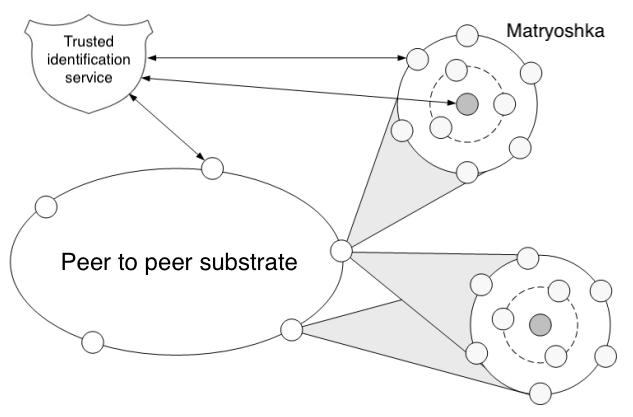
\includegraphics[width=3in]{matryoshka.png}
\caption{System Overview \cite{4801860}}
\label{fig: matryoshka} 
\end{center}
\end{figure}
The system has three main components:
\begin{itemize}
\item \textbf{Several Matryoshkas:} It is a network of concentric nodes which provides the basic distributed structure used to store user data.
\item \textbf{A peer to peer substrate} like a Distributed Hash Table provides global access to a user's data based on his identifiers.
\item \textbf{A trusted Identification service} which guarantees authentication.
\end{itemize}
Figure \ref{fig: matryoshka} shows an overview of the system.
A user forms a matryoshka when it first joins the network. The user is at the core of the rings. The first ring surrounding the user is used to replicate data. These nodes are the ones that the user directly trusts, and they serve the request of the user's data if permitted to do so. The nodes in the first ring trust the nodes in the second ring, and so on. Data requests start from the outermost ring of the user's matryoshka and reach to the innermost. Exchange of requests takes place only between those nodes which trust each other. These nodes are not necessarily directly trusted by the user. The trust relationship is on a hop-by-hop basis. The user can selectively encrypt data and share the keys with nodes it trusts. Public data is encrypted with a key that is shared with everyone. Private data is encrypted with a key that is shared only with the nodes that the user directly trusts. Every node keeps updating its matryoshka with time.\\
The distributed peer to peer network is used to route the request for the user's data to the outermost ring of the proper matryoshka.
The Identification service provides identifiers and certificates to each node for authentication.\\
This is a very novel solution to preserve the user's privacy. It also has all the other advantages of a decentralized system. However, it is still a work in progress. There is a need to improve key management, forward secrecy, backward secrecy, and key revocation mechanisms.

\subsection{Countering Fake News}
Taiwan has a very innovative system set up to combat the spread of fake news \cite{co-facts}. Each ministry has a team that observes social media posts and looks for disinformation campaigns going on. Once they discover such campaigns, they are in charge of making an equally or more convincing narrative against the fake news within 60 minutes. It could be a short film, a social media post; ministers live stream, standup comedy, or anything else that can go viral. The clarifications are spread through the president's deputy minister's accounts on multiple social media platforms. The followers are asked to spread the information.
\par
However, it cannot counter disinformation which spreads on end to end encrypted platforms. These platforms are like closed echo chambers. For this purpose, they developed a technical solution called co-facts. It was developed with LINE and Facebook. Following is the working of the system.
\begin{itemize}
\item If someone suspects spam or disinformation is spreading in such channels, they forward the message to a bot called CoFact on the LINE app.
\item The Line bot then checks the database to see if the message has been fact-checked before. If so, the earlier recorder reply is sent to the user.
\item If-not, the message is recorded in the database, and it shows on the fact-checking website to an editor.
\item Editors are people who have signed up to volunteer for the service. An editor reads the message, and fact checks it through relevant sources like google or internal ministry.
\item Then he adds a response stating whether the message is true or false.
\item This message then gets added to the database and sent to the user through the chatbot.
\end{itemize}

\subsection{vTaiwan And Pol.is}
The Taiwan government has an innovative solution to make decisions with people’s consensus \cite{polis}. The government invited activists to create a platform to better communicate with the youth. Gov zero (g0v); a tech civic community created a platform called vTaiwan in 2015 and still runs it.The platform enables citizen, civil society organizations, experts and elected representatives to discuss proposed laws via its website as well as face to face meetings and hackathons. The goal is to help policymakers make decisions that gain legitimacy through consultation
v-Taiwan relies on a lot of open-source tools for soliciting proposals, sharing information, and holding polls, but one of the key parts is Pol.is
\begin{itemize}
\item On Pol.is a topic is put up for debate.
\item Anyone who creates an account can add a comment
\item People can upvote or downvote others comments
This sounds much like other online forums but there are 2 main differences
  \begin{itemize}
    \item Users cannot reply to comments - This stops trolls
    \item It creates a map of all the participants in the debate using the upvotes and downvotes, clustering the people who have voted similarly
  \end{itemize}
\item Although there may be thousands of separate comments, like-minded groups rapidly emerge in this voting map, showing where there are divides and where there is consensus.
\item People then naturally try to draft comments that will win votes from both sides of a divide, gradually eliminating the gaps
\end{itemize}
Example of the platform's success
\textit{Topic: How to regulate the ride-hailing company Uber ?}
As new people joined the debate - the comments ranged from
\begin{itemize}
\item Calls to ban uber
\item Subject it to strict regulation
\item Let the market decide
\item Uber has a dynamic business model which can create a lot of jobs
\end{itemize}
Within a few days, two groups emerged - Pro-Uber and Anti-Uber (twice as large). But as the groups sought to attract more supporters, members started posting comments on matters that everyone could agree were important such as rider safety and liability insurance. Gradually they refined them to get more votes\\
The end result was a set of seven comments that enjoyed almost universal approval  like
\begin{itemize}
  \item The govt should set up a fair regulatory regime
  \item Private passenger vehicles should be registered
  \item A for-hire driver must be able to join multiple platforms
\end{itemize}
Thus The divide between pro and anti uber camps had been replaced by consensus on how to create a level playing field for Uber and Taxi firms and create more competition
\subsection{Protocol Buffers}
XMPP uses XML for data serialization which is too verbose.  XML is stored as a text file hence it is large in size. An alternative to XML can be Google’s protocol buffer \cite{prot-buff}. It is a platform-independent, language-neutral and extensible mechanism for serializing data. The structure of the data is defined using protocol buffer message types in  \textit{.proto} files.  A simple example of a \textit{.proto} file is as follows: 

\begin{figure}[H]
\begin{center}
  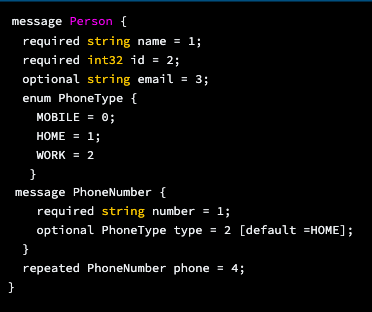
\includegraphics[width=3in]{proto_file.png}
  \caption{A simple proto file structure.\cite{prot-buff}}
\end{center}
\end{figure}

After defining the data you compile the file in your required language. The compiler generates cla	sses in that language to access the data programmatically. Supported languages are Java, Python, Objective-C, C++ and more. An example of how the above defined data will be stored and accesses in C++ is as follows:
\begin{figure}[H]
\begin{center}
  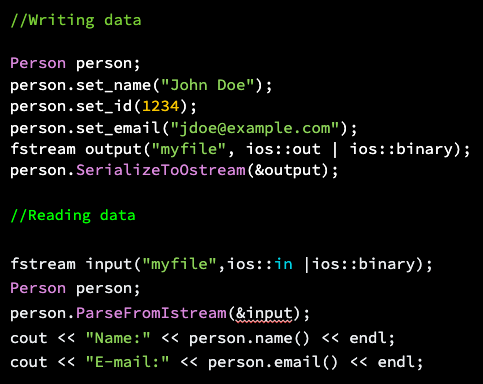
\includegraphics[width=3in]{access_data.png}
  \caption{Accessing the data.\cite{prot-buff}}
\end{center}
\end{figure}

Accessing the data is much simpler than parsing XML or any other data format. The file generated is smaller in size than XML since it is a binary file. This makes protocol buffer faster. It is also easier to use programmatically. Thus it is an ideal replacement of XML. 
\subsection{SIGNAL}
SIGNAL is an open-source project which aims at providing instant messaging with complete end-to-end encryption. Many applications nowadays offer end-to-end encryption, so what is unique about SIGNAL?. Companies claim that since the messages are end to end encrypted, they cannot read the user's message contents. While this may be true, we cannot trust the company with metadata.  Companies can still read the metadata and extract analytical information from them. Also, companies do not allow outside researchers to inspect their data collection process or code of their messaging apps. This means we need to trust them by taking their word that it's not collecting our data. Signal also encrypts virtually all of the metadata, including who sent the message. Only the person who receives the message knows who sent the message. And Signal is open-source. Anybody can look into its code and verify its security features. The app is maintained and developed by the Signal Foundation, a non-profit organization. Signal uses some very complex and secure encryption algorithms based on the Off-the-Record(OTR) protocol.\\
\textbf{Off-the-record Protocol:} It is a security protocol which aims to protect user privacy. An important feature of the protocol along with usual confidentiality, integrity and authentication is deniability, i.e. Nobody can claim that a particular message was sent by someone, not even the person to whom it was sent. 
\begin{figure}[H]
\begin{center}
  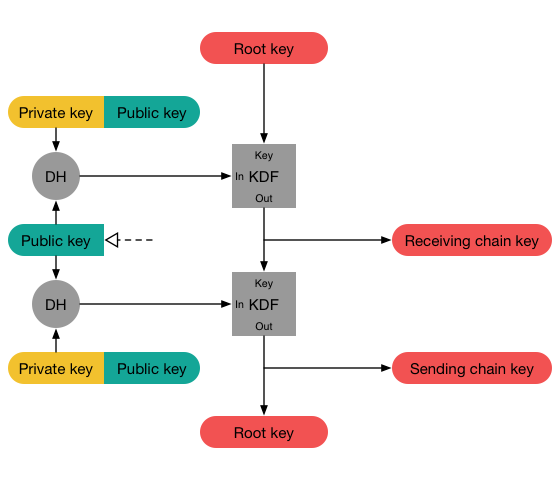
\includegraphics[width=3in]{double_ratchet.png}
  \caption{Generating keys from the DH ratchet.\cite{signalDoc}}
\end{center}
\end{figure}
Singal protocol uses two keys for encryption. One for each direction. If Alice communicates with Bob, then Alice has a sending key with which she encrypts the message. The sending key of Alice is the same as the receiving key of Bob, using which he can decrypt
the message. Similarly, Bob has a sending key, which will be the same as Alice's receiving key. \\ 
The keys are derived using a Key Derivation Function (KDF) that is similar to a one-way hash function. One of the inputs to the KDF is the previous key, and another input is a secret key. This secret key is generated using a variant of Diffie Hellman key exchange. 
These keys are changed whenever there is a change in the direction of the messages. Each side generates the keys locally using the KDF chains. The Diffie Hellman secret is also changed occasionally. (usually for every message) Thus there are three chains, The Diffie Hellman chain, The sending chain, and The receiving chain. This concept of generating keys locally using a shared secret is known as ratcheting. There are two ratchets in this design, the Diffie Hellman ratchet, and the sending/receiving ratchet. Thus it is also known as the Double Ratchet Algorithm. This hash like property of the KDF chain ensures forward secrecy (i.e., cannot derive past keys from a key ), and The Diffie Hellman ratchet provides backward secrecy (i.e., cannot derive future keys from a key).
The details of the signal protocol are available at \cite{signalDoc} \\
Signal is a very secure and open source security protocol which is also used by the famous messaging giant Whatsapp.      
\section{Conclusion}  
\label{SEC: conclusion}
Through this survey, we were able to find out more about the current situation of open messaging standards in the industry. Open messaging standards are important for interoperability and they also enable more privacy for the user.  XMPP was designed to provide interoperability to instant messaging applications. RCS aims to bring back the glory of SMS days to the telecom operators and in the process provide interoperability. The Signal open-source project provides a higher level of user privacy. The SOLID ecosystem tries to decentralize data ownership. These systems have one or more qualities of an ideal open messaging system that we envisioned before surveying them. 
\par
Designing an open standard with all the ideal characteristics is a complex process. The following practical points need to be considered while doing so
\begin{itemize}
\item User adoption
\item Motivation for companies to support the standard. 
\item A business model
\item Security and Privacy
\item Decentralization of the system
\item A federation to regulate the system. 
\end{itemize}
\par
Companies usually do not support a system unless they have a strong motivation behind it. The motivation can be to gain trust from users, earn capital, or establish a brand name for the company. XMPP which was one of the first shots at interoperability failed due to companies turning towards their proprietary solutions. Interoperability was not high on the agenda of these companies. Companies want to gain market dominance. Hence the first step towards designing an open system of instant messaging is to convince major players in the industry to support the system. \\
An open system should be secure. It should not compromise the privacy of the user at any cost. Hence it should support end-to-end encryption. It should also encrypt as much metadata as possible. User privacy is essential and a key element in gaining users’ trust. The signal protocol is an ideal example of a secure system.  
An open system should not be dependent on a single organization. It should be supported by a federation of organizations. It should be independent of the platform being used. RCS and E-mail have these properties. 
An open system should control user data in a responsible manner. It should only store the data which is essential to provide the service to the user. All other data which may contain sensitive information should only be stored on the user's device (like chat history) or on decentralized systems like SOLID.  
Also, the system must support performance by using compact serialization techniques. For example, using Google’s protocol buffer instead of XML. It is simpler, smaller, faster, and less ambiguous. Also, it is easier to use programmatically. 
The open system should also provide a way to stop the spreading of fake news. Features like the LINE bot that we discussed should be incorporated. The system should be designed to be mobile-first,        i.e. optimized for wireless mobile communication. 
We have discussed several systems which have a subset of the properties required in an open messaging standard. I conclude that in order to build such a system one has to consider all these aspects and think of how to proceed further.

\section{Acknowledgement}
\label{SEC:acknowledgement}
This survey was done under the guidance of Prof. Kameswari Chebrolu and Prof. Bhaskaran Raman. I thank them for their valuable guidance and feedback during the survey.



\newpage
\nocite{*}
\printbibliography
\end{document}          
